\documentclass[conference]{IEEEtran}
\IEEEoverridecommandlockouts

\usepackage{cite}
\usepackage{amsmath,amssymb,amsfonts}
\usepackage{algorithmic}
\usepackage{graphicx}
\usepackage{textcomp}
\usepackage{xcolor}
\usepackage{csvsimple}
\usepackage{rotating}
\usepackage{subfig}
\usepackage{float}
\usepackage[toc,page]{appendix}
\usepackage{url}
\usepackage[capposition=top]{floatrow}
\usepackage[skip=8pt,font=scriptsize]{caption}

\usepackage{listings}
\usepackage{color}

\definecolor{dkgreen}{rgb}{0,0.6,0}
\definecolor{gray}{rgb}{0.5,0.5,0.5}
\definecolor{mauve}{rgb}{0.58,0,0.82}

\lstset{frame=tb,
	language=Java,
	aboveskip=3mm,
	belowskip=3mm,
	showstringspaces=false,
	columns=flexible,
	basicstyle={\small\ttfamily},
	numbers=none,
	numberstyle=\tiny\color{gray},
	keywordstyle=\color{blue},
	commentstyle=\color{dkgreen},
	stringstyle=\color{mauve},
	breaklines=true,
	breakatwhitespace=true,
	tabsize=3
}

\usepackage{wrapfig}
\usepackage{lscape}
\usepackage{rotating}
\usepackage{epstopdf}
\usepackage{array}
\usepackage{makecell}
\renewcommand\theadalign{bc}
\renewcommand\theadfont{\bfseries}
\renewcommand\theadgape{\Gape[4pt]}
\renewcommand\cellgape{\Gape[4pt]}



\def\BibTeX{{\rm B\kern-.05em{\sc i\kern-.025em b}\kern-.08em
		T\kern-.1667em\lower.7ex\hbox{E}\kern-.125em}}
\graphicspath{ {fig/} }


\begin{document}
	
	\title{Simulation and Analysis of a Wireless Sensor Network using Message Passing Interface }
	
	\author{
		\IEEEauthorblockN{Samarasekara Vitharana Gamage, Bhanuka Manesha}
		\IEEEauthorblockA{	bsam0002@student.monash.edu \\28993373}
		\IEEEauthorblockA{\textit{School of Information Technology} \\
			\textit{Monash University}\\
			Malaysia}
		}
	\maketitle
	
	\begin{abstract}
		
	\end{abstract}

	
	\begin{IEEEkeywords}
	
	\end{IEEEkeywords}
	
	\section{Introduction}
	
	The rapid growth of IoT devices and sensors has led to a high demand in efficient sensor architectures \cite{othman2012wireless}. Since sensors mainly run on embedded devices and battery powered systems, the need for power efficient architectures are on the rise \cite{guy2006wireless}. Currently Wireless Sensor Network (WSN) architectures are the standard for low power sensor networks. To accomplish low power usage each node in the WSN can only communicate with the four adjacent nodes and the base station. In order to implement these WSNs, highly efficient Inter Process Communication (IPC) architectures are needed.
	
	An Inter Process Communication is a system that allows data to be communicated between two processes \cite{techopedia.com}. Pipes, Socket, File, Signal, Shared Memory and Messege Queue are few of the different IPC architectures currently available \cite{onsman_2018}. Since, any given node has to communicate with either another node or the base station and the nodes can be located in different geographical locations, out of the given architectures, the socket architecture will be the most suitable as it creates end points on each node to send and receive data. There are different design space architectures for socket based IPC architectures such as hyper cube, pyramid, tree and grid (nearest neighbor). But since a sensor node can only communicate with the four adjacent node i.e. nearest neighbors, a grid based socket IPC architecture would be the best method for the WSN. 
	
	Another constraint of WSNs, is that not only the have to operate on low power, but also be secure enough to broadcast sensitive data wirelessly. This is a major concern as most of the communication is done wirelessly and attackers can get the data easily \cite{wn}. To achieve this efficient encryption standards are used by the system.
	
	In the following sections, we explore and analyze a grid based IPC architecture that uses state of the art encryption standards and can run efficiently on a Wireless Sensor Network.
	
	
	
	
	\section{Theoretical Analysis and Inter Process Communication Design}
	
	The Inter Process Communication Design used by the WSN is discussed in this section. The Wireless Sensor Network uses a grid based architecture where each node is able to communicate with the adjacent node and the base station only.
	
	
	\subsection{ Inter Process Communication Grid Architecture}\label{IPCArc}
	
	The number of nodes used by the WSN  depends on how many processes are allocated by the user at the start. If the user specifies the number of nodes as 21, then the system uses one node as the base and the rest as the sensor nodes. Using MPI we allocate rank $0^{th}$ process to the base station and the rest of the nodes as the sensor nodes. 
	
	The system uses a dynamic grid based architecture. So the layout of the nodes are based on the height and width specified by the user. Figure \ref{gridlay}  illustrates a simple example of how the user can rearrange a 21 node architecture. Figure \ref{gridlay1} illustrates how the grid is initialized when the width is 4 and height is 5, while Figure \ref{gridlay2} illustrates when its 2 and 10 respectively.
	
	
	\begin{figure*}[!t]
		\centering
		\caption{Dynamic Grid Layout}
		\subfloat[4 X 5 grid]
		{
			\centering
			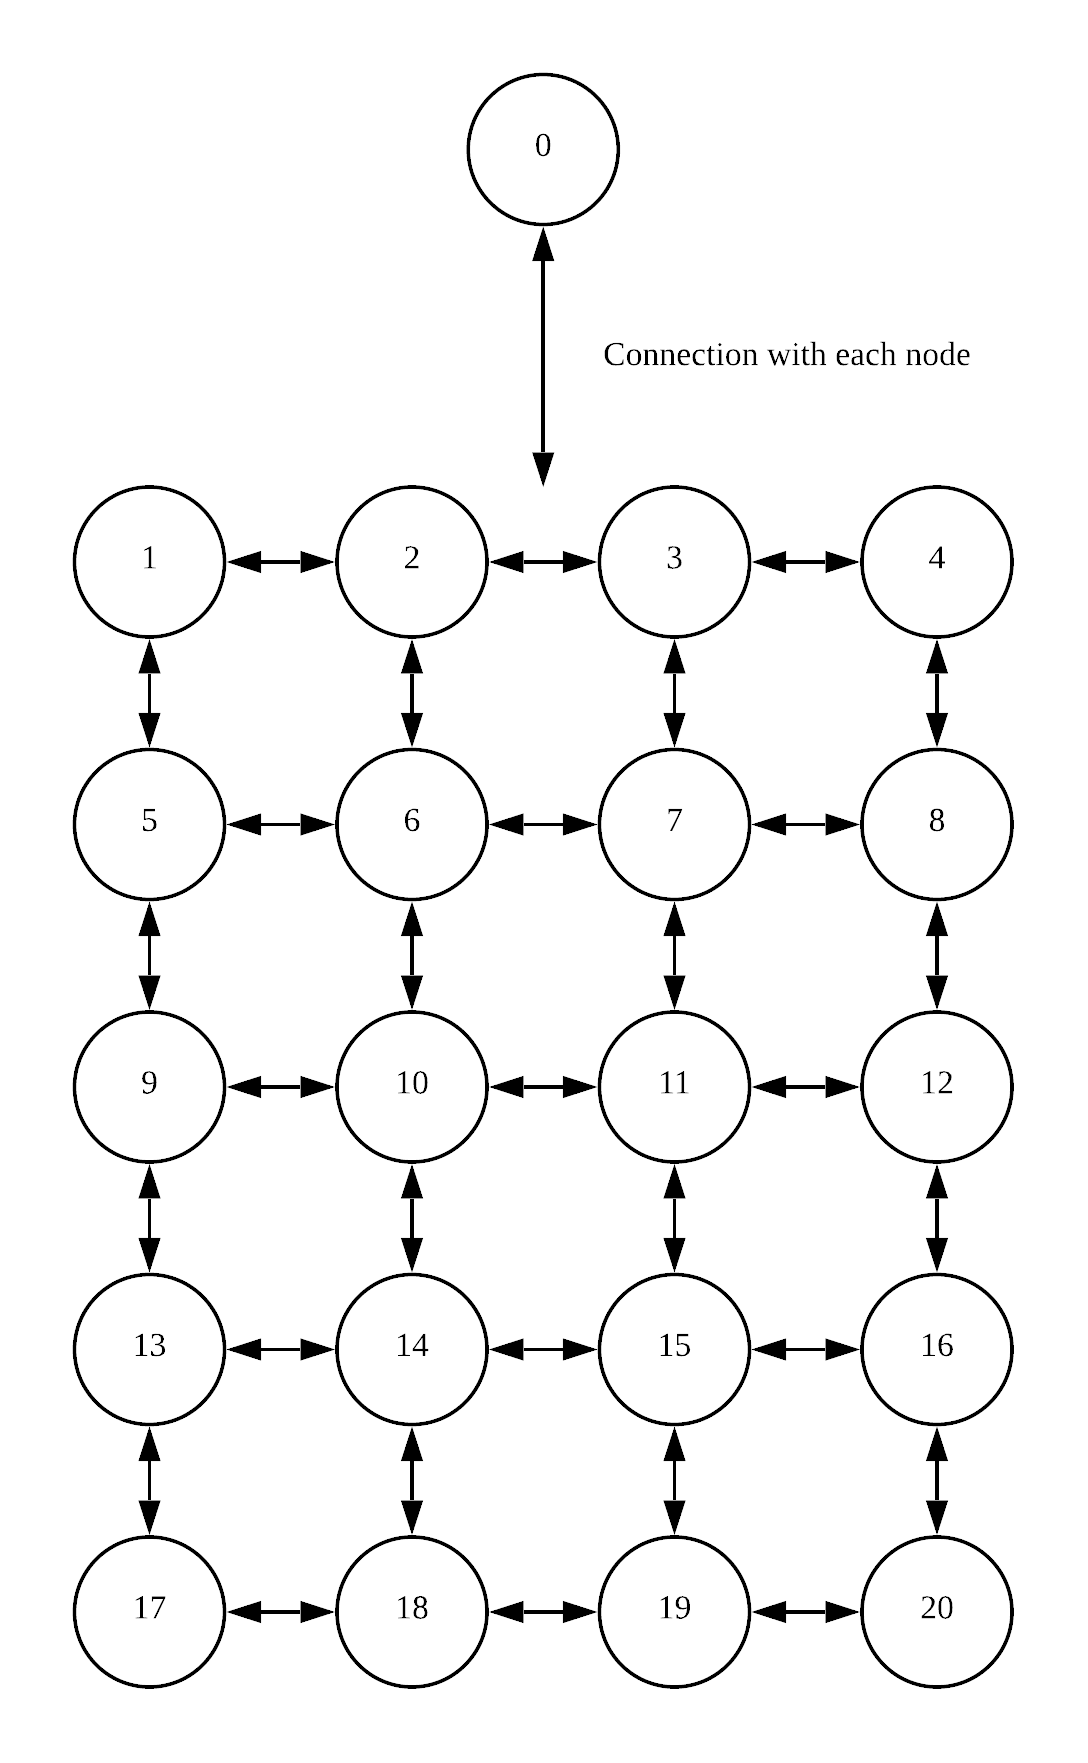
\includegraphics[width=2in]{grid1}
			\label{gridlay1}
		}
		\\
		\subfloat[10 X 2 grid]
		{
			\centering
			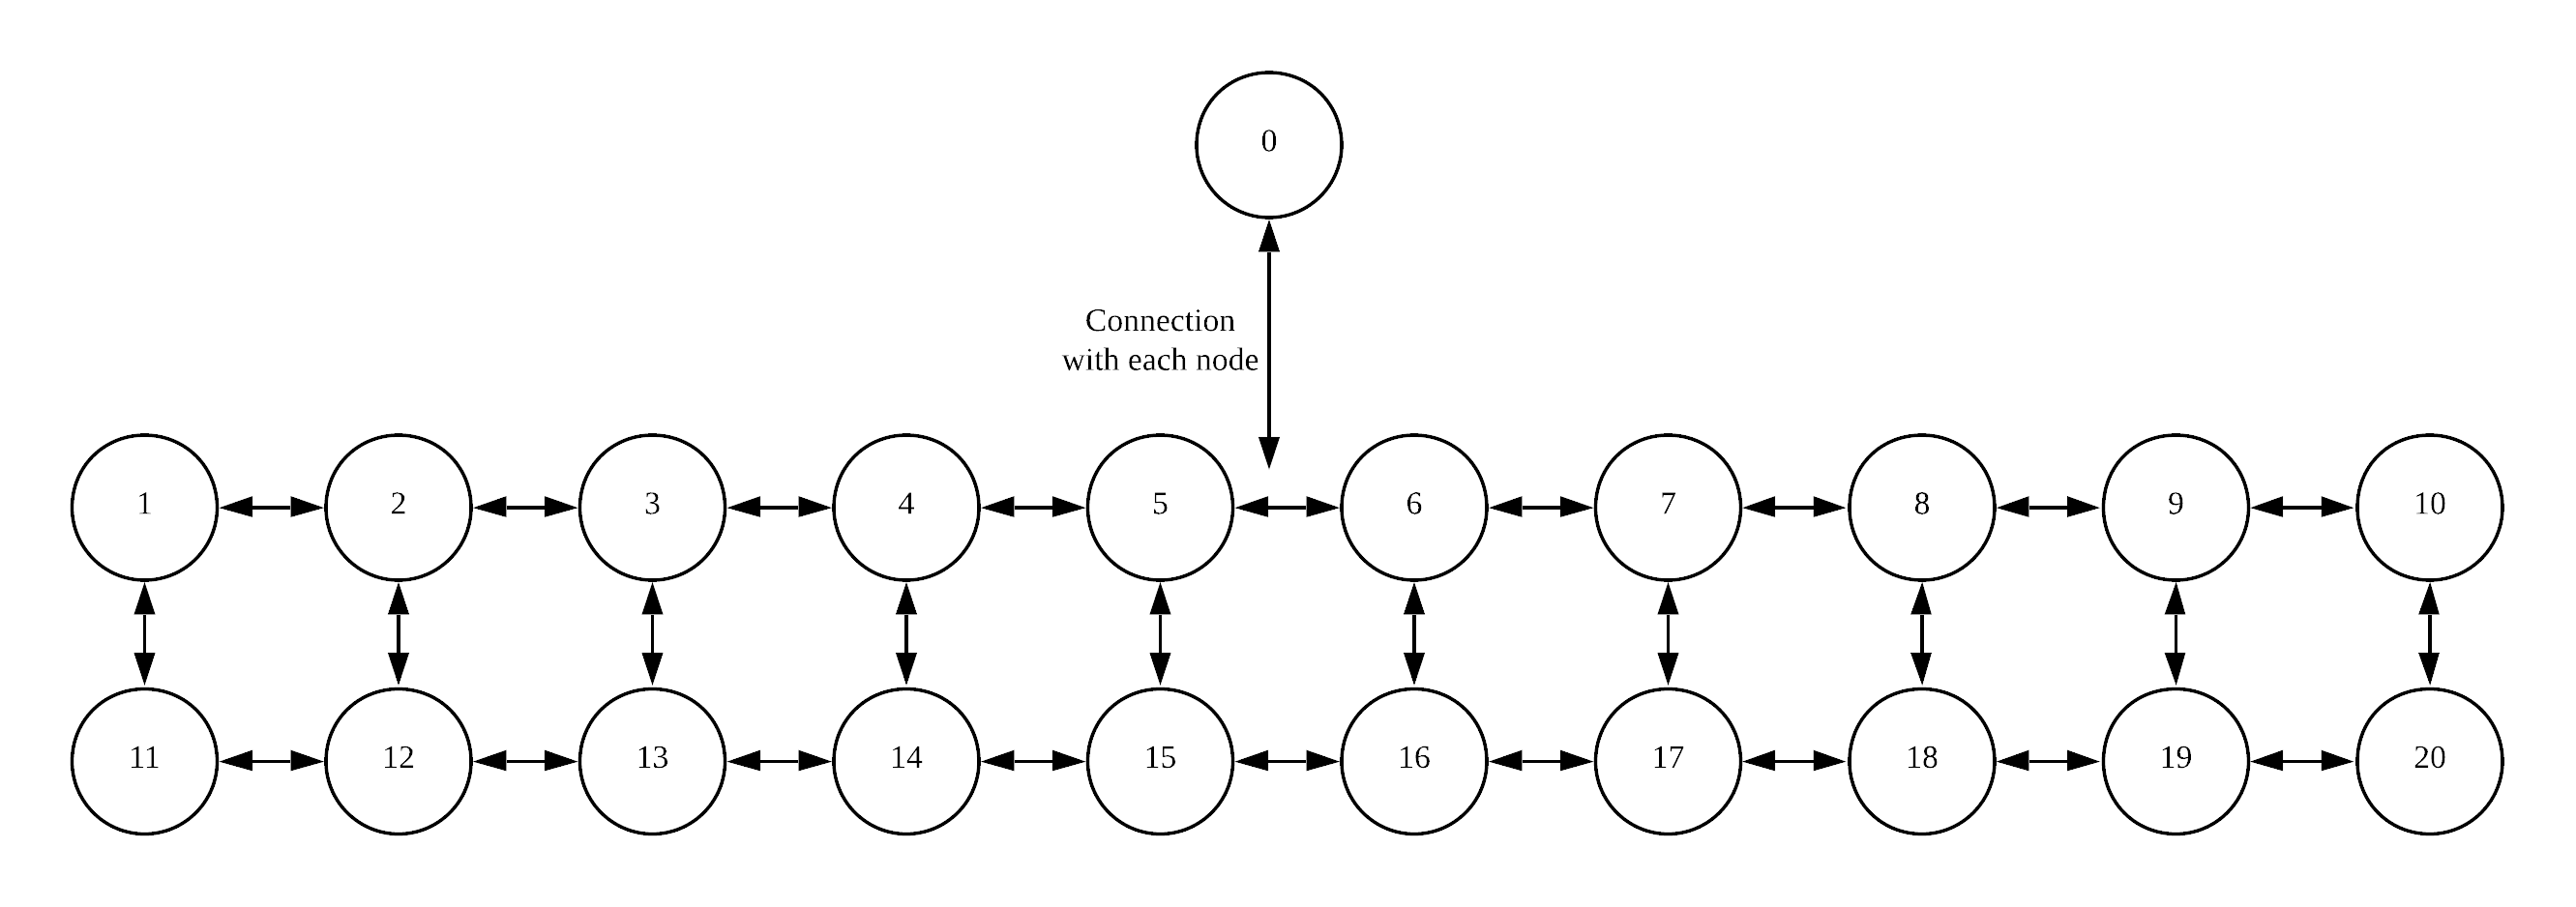
\includegraphics[width=6in]{grid2}
			\label{gridlay2}
		}
		\label{gridlay}
	\end{figure*}
	
	
	After initializing, each node is able to communicate with the adjacent four nodes i.e left, right, top and bottom nodes and also with the base station. The base station is able to communicate with each node individually. The adjacent nodes of each of the sensor nodes are calculated using the height and width specified by the user. Equation \ref{row} and \ref{col} can be used to determine the row index and column index of a given node in the WSN. \emph{Do note that we first minus 1 from the current rank, this is due to the base station being rank 0.}
	
	
	\begin{equation}
	row index = (rank - 1) \, // \, width
	\label{row}
	\end{equation}
	
	
	\begin{equation}
	column index = (rank - 1) \ mod \ width
	\label{col}
	\end{equation}
	
	After determining the row index and the column index, we can use Equations \ref{left}, \ref{right}, \ref{top} and \ref{bottom} are used to get the four adjacent nodes. 
	
	\begin{equation}
	left = row index \times width + column index
	\label{left}
	\end{equation}
	
	
	\begin{equation}
	right = row index\times width + column index + 2
	\label{right}
	\end{equation}
	
	\begin{equation}
	top = (row index - 1) \times width + column index + 1
	\label{top}
	\end{equation}
	
	
	\begin{equation}
	bottom = (row index + 1) \times width + column index + 1
	\label{bottom}
	\end{equation}
	
	Note that the shift in the ranks due to base station is in rank 0 is accounted for in the equations and also a check needs to be done to ensure that the current rank is not an edge or corner node. Using this process, we do not need to send the rank values to the base station when an event occurs. The base station can use the rank of the incoming node to generate the four adjacent nodes in order. Therefore this reduces the message size and optimizes the nodes to use less energy and the base to consume more energy for computation.
	

	Published papers..
	
	
	\begin{figure*}[!ht]
		\centering
		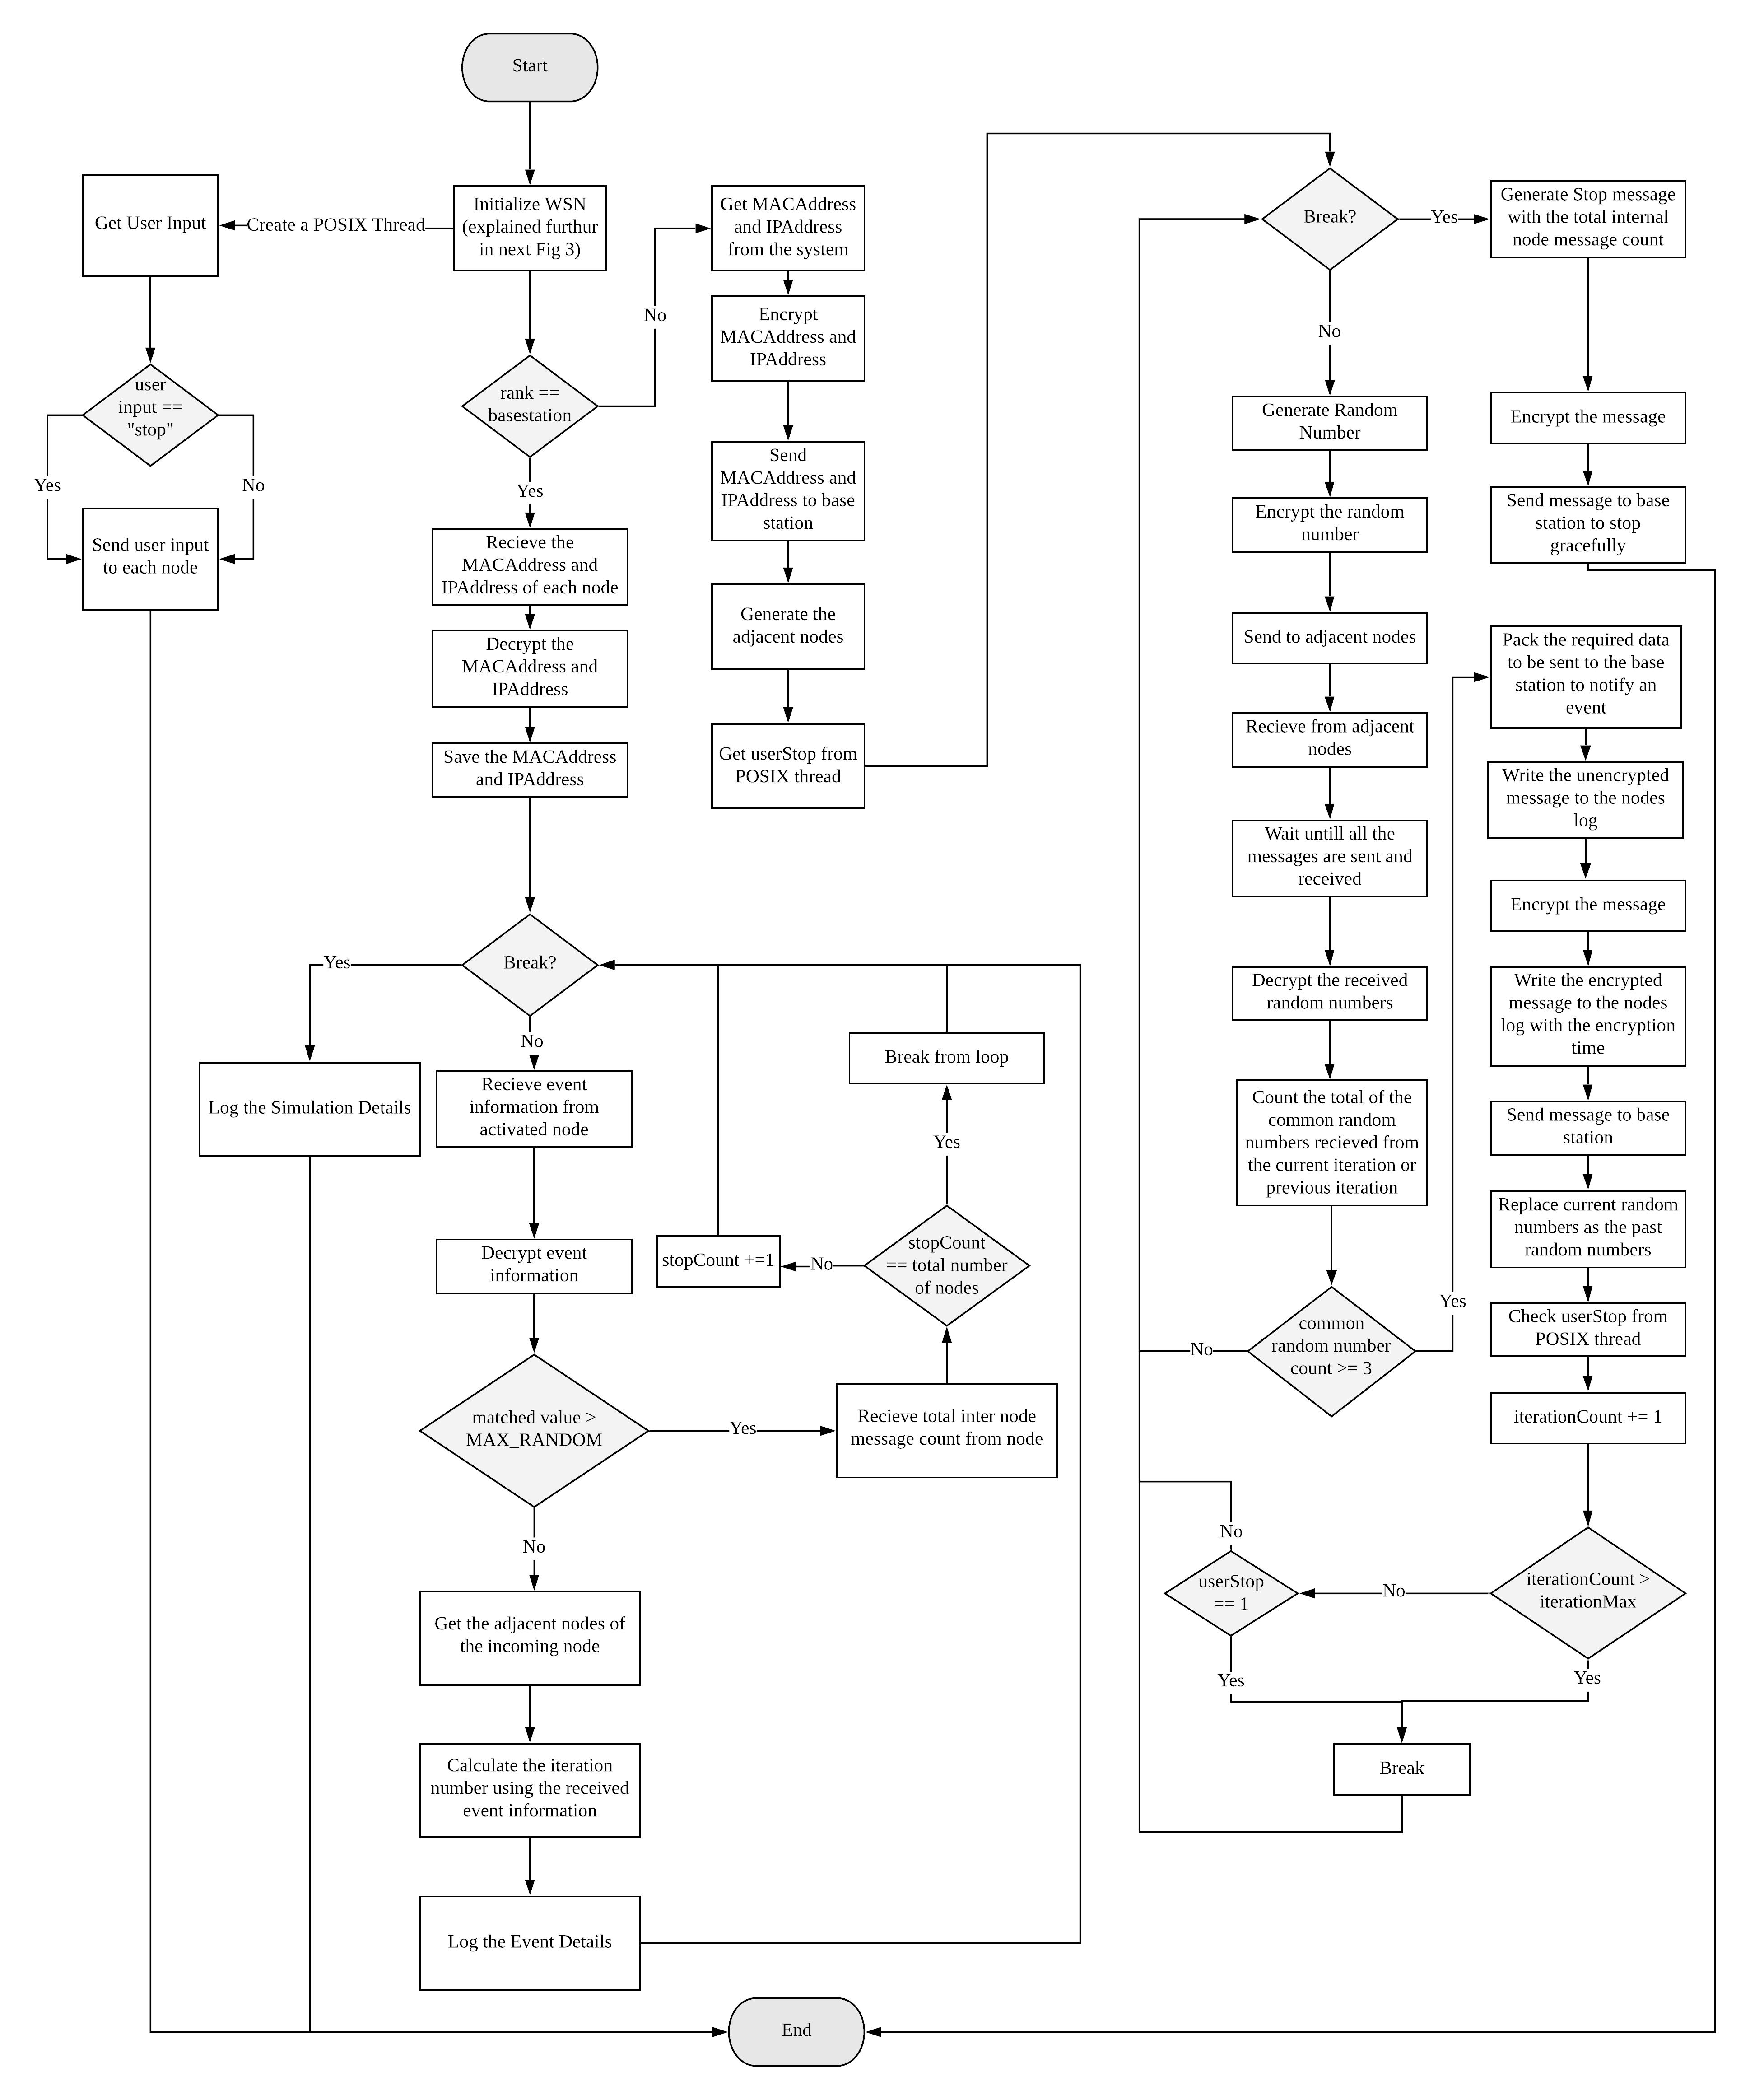
\includegraphics[width=6in]{arc}
		\caption{Technical Flowchart for WSN Inter Process Communication}
		\label{arc}
	\end{figure*}
	
			\begin{figure}[!ht]
		\centering
		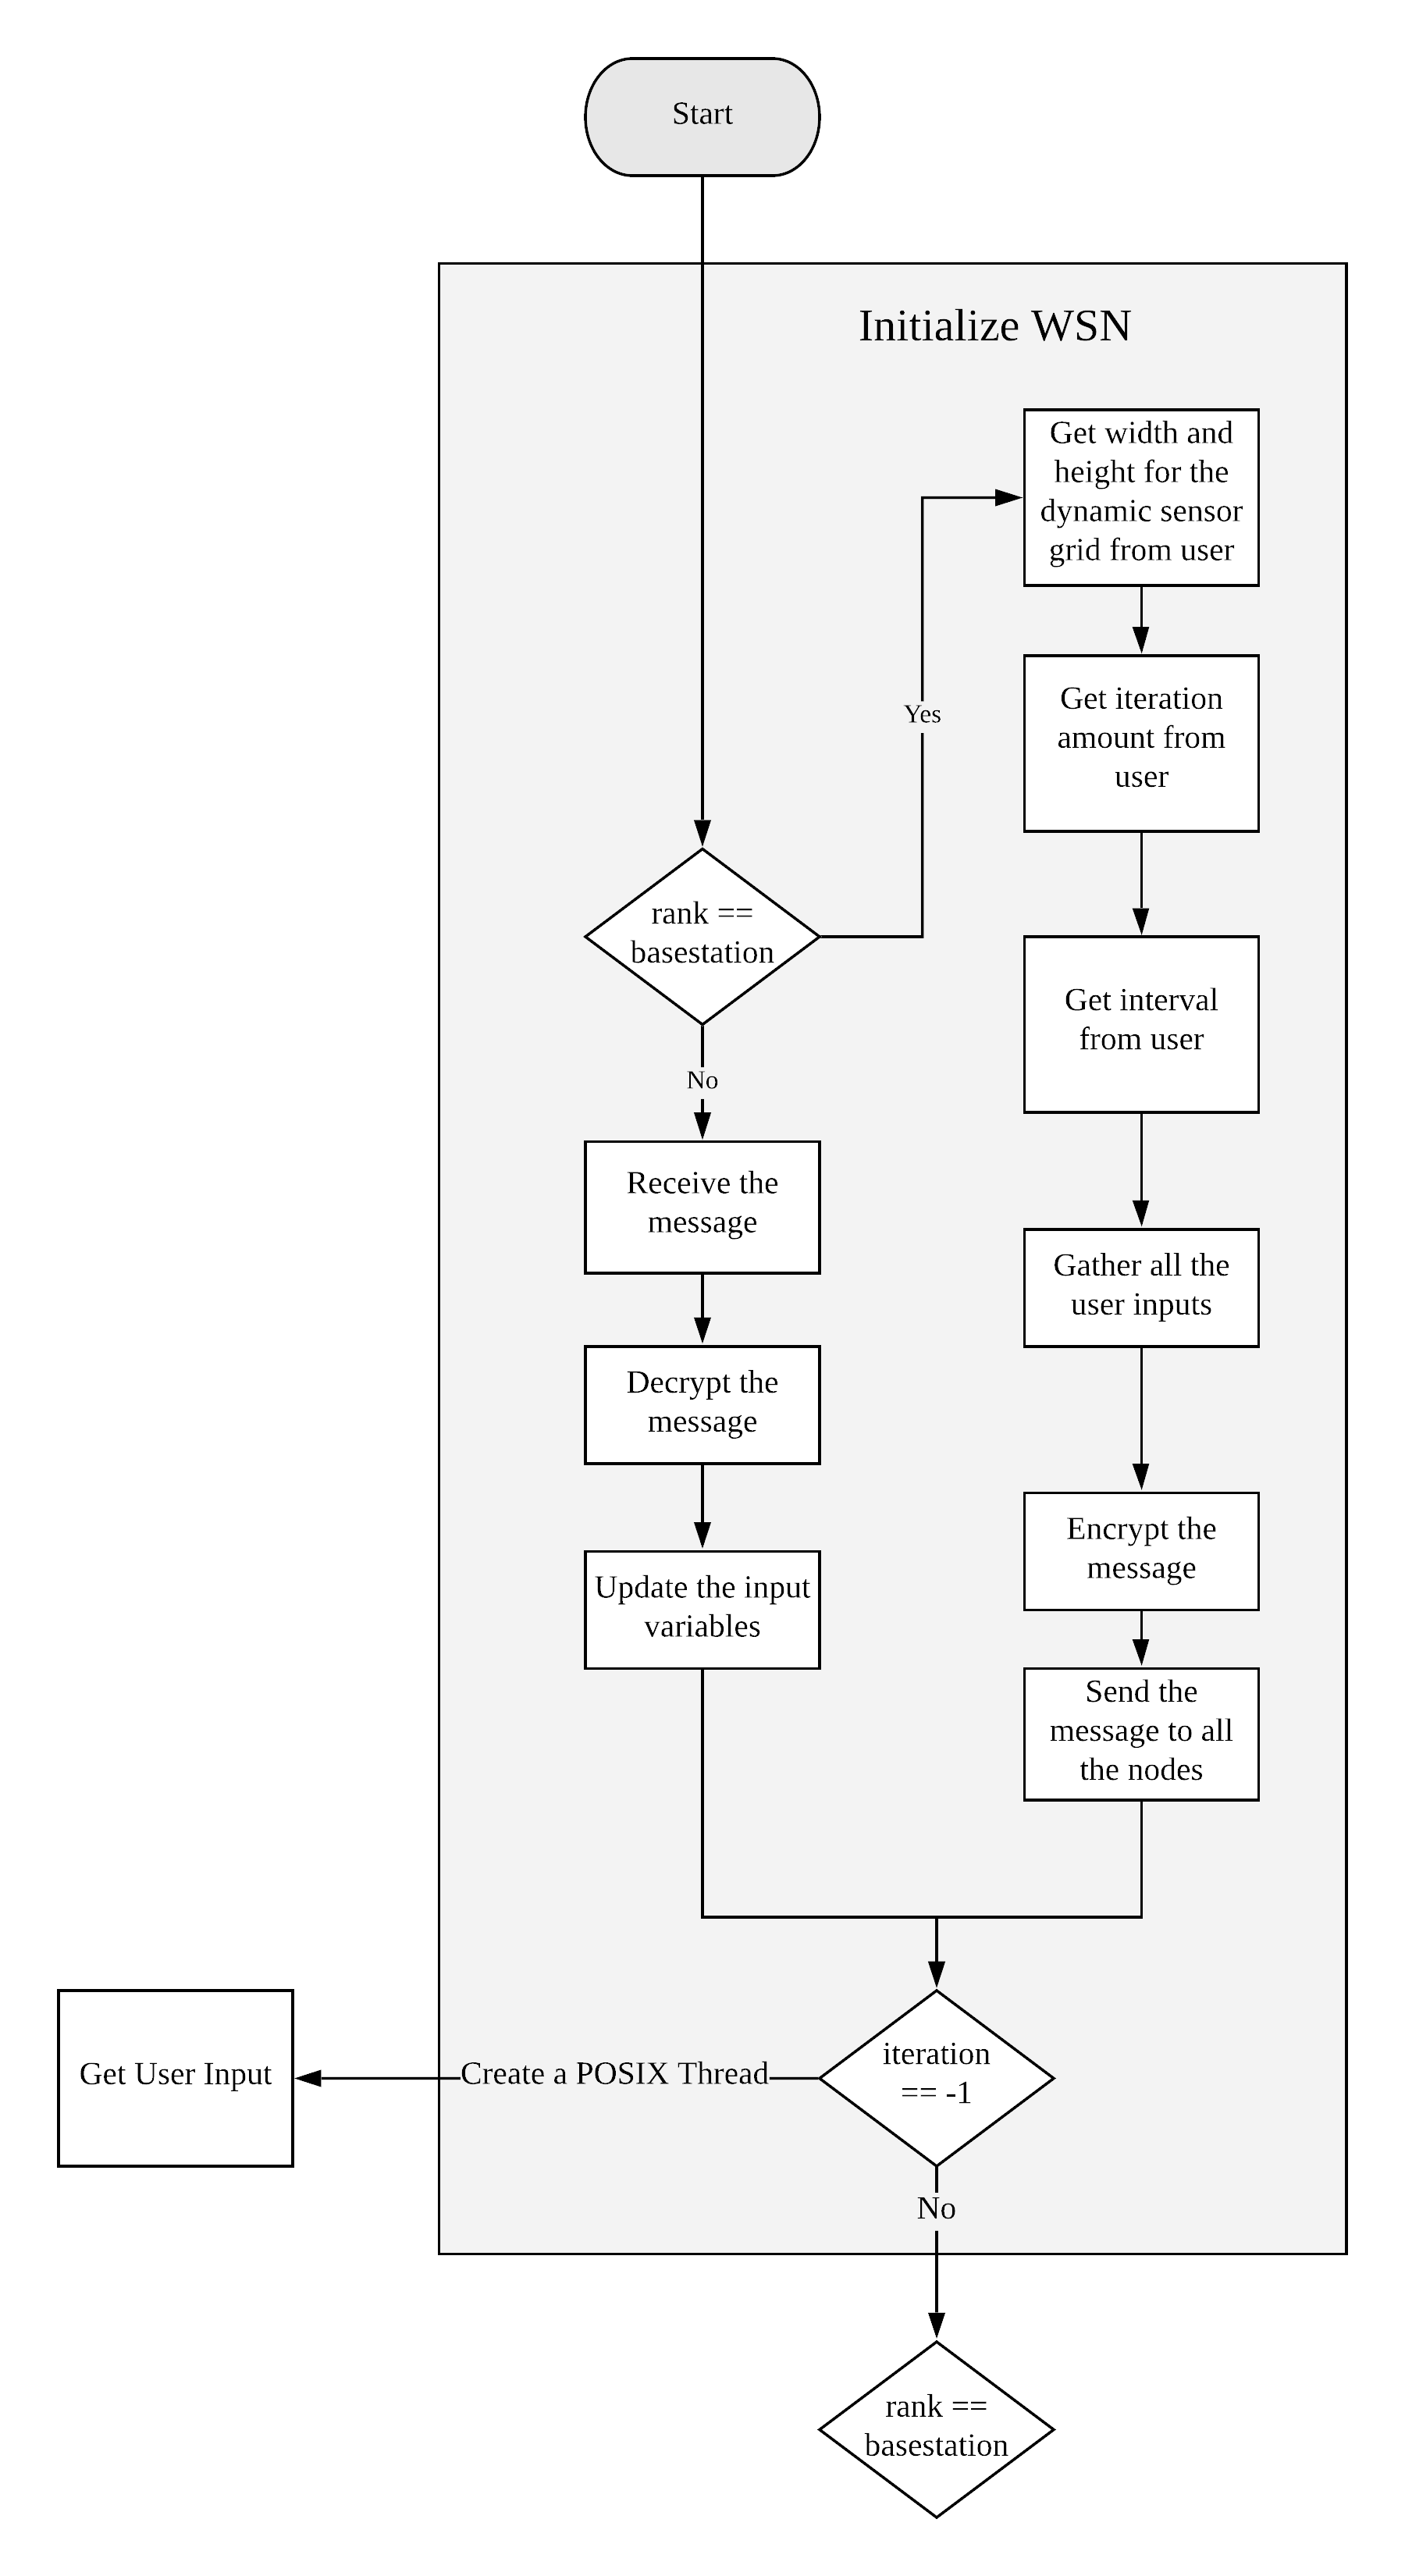
\includegraphics[width=3in]{inWSN}
		\caption{Technical Flowchart for Initializing the WSN}
		\label{inWSN}
	\end{figure}
	
	
	\subsection{ Wireless Sensor Network Event Detection Algorithm }
	
	
	Now we look into the algorithm used by the system to detect events in the WSN. The system is divided into two main sections.
	
	\begin{itemize}
		\item Base Station which logs all the events
		\item Sensor Nodes which triggers and checks for events
	\end{itemize}

	Initially the system generates sensor network grid dynamically using the \emph{width} and \emph{height} given by the user which was discussed in Section \ref{IPCArc}. Then both the sensor nodes and the base station start running their respective methods. First the IP Address and the MAC Address is sent from each node to be stored in the base station for logging purposes. These messages are encrypted using the AES encryption algorithm discussed in section \ref{encryption}. The base station will then decrypt the message and store it in a dynamic array. Below is the data passed from the node to the base station when initializing the system.
	
		\begin{itemize}
		\item IP Address of the node
		\item MAC Address of the node
	\end{itemize}
	
	Now let us look into the algorithms used by the sensor nodes and the base station to generate and detect events.
	
	\subsubsection{Sensor Nodes}
	
	Firstly, each node generates a random number and sends it to the adjacent nodes. This message which contains the random number, sent between the nodes are also encrypted. Then the sensor node starts receiving random numbers from the adjacent nodes. If three or more random numbers are the same, an event is detected. The algorithm also takes into account the random numbers generated by the nodes in the previous iteration. So it works as a sliding window with a time frame depth of 2. Then the nodes will notify the base station by sending a message. This message contains the following details:
	
		\begin{itemize}
		\item The random number that triggered the event
		\item An array of four elements which corresponds to the iteration of the matched value. If the left adjacent node matched with the random number of the previous iteration, the array will contain the iteration number of the previous element in the $0^{th}$ index of the array. 
		\item The MPI Wtime of the event detection to be used to calculate the communication time
		\item The date time string of the time when the event was detected to be used for logging
	\end{itemize}
	
	After sending the message to the server, it saves the random numbers from the current iteration. If the maximum number of iterations is reached or the users stop signal is received, the node will send a termination signla to the base station to exit out of the system gracefully.
	

	\subsubsection{Base Station}
	After the WSN is initialized, the base station starts checking for messages from any node. If the user has entered -1 as input for the iteration, the system will terminate checking for events only if user enters the keyword "stop". In order for this to work, the base station creates a POSIX thread, which enables it to check for user inputs as well log the events from the nodes. When the user inputs the keyword "stop", the thread then sends a message to the nodes to stop event detection gracefully. Then the nodes will start sending the termination messages back to the base station and the system will shut down.
	
	Figure \ref{arc} breaks down the algorithm of the whole system in to a technical flowchart. Then Figure \ref{inWSN} explains how the system initializes the WSN, based on the dynamic user inputs.
	
	
	Blocking and Non Blocking Send
	
	
	\subsection{ Encrypting communication and its effects }\label{encryption}
	
	Due to the increase risk of cyber attacks, all wireless networks needs to be encrypted as its is easier to attack and steal unencypted data. So, all the messages are encrypted throughout the wireless sensor network. After comparing multiple encryption standards, Advanced Encryption Standard (AES) was used to encrypt the messages.
	
	AES is a symmetric block cipher which can encrypt and decrypt information \cite{rouse_cobb}.The Encryption part of the algorithm converts data into cipher text form while decryption part converts cipher text into text form of data.  AES used different 128/192/256 bit keys to encrypt and decrypt data. For the WSN implementation we will be using AES 192, which uses a 192bit key. Since AES is the current standard for wireless communication, financial transactions and e-business we will be using it instead of other encryption algorithms \cite{rfwirelessworld}. Block Cipher has many modes of operations. Since AES is also a block cipher, it has many modes of operations. Examples for these are Electronic Codebook (ECB), Cipher Block Chaining (CBC), Cipher Feedback (CFB) and Counter (CTR) \cite{meghna_2019}.
	
	\begin{figure}[!h]
		\centering
		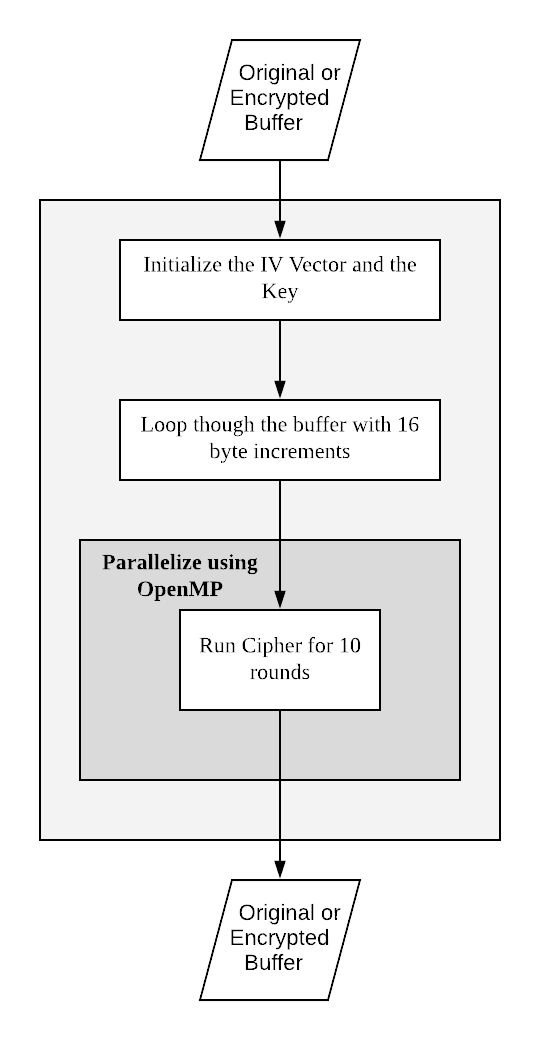
\includegraphics[width=2.3in,keepaspectratio]{encdec}
		\caption{Encryption and Decryption algorithm with OpenMP}
		\label{encdec}
	\end{figure}	

	For the WSN, we will be using the tiny-AES online implementation by kokke \cite{kokke_2019}, which use the Counter (CTR) block cipher mode. In order to improve the speed of the encryption process we will be using OpenMP \cite{openmp_2018} to parallelize the process. This implementation uses the same method to encrypt and decrypt the buffer. Since the AES implementation encrypt and decrypt a block size of 16 bytes for 10 rounds, OpenMP is applied on the inner loop. So the 10 rounds are done in parallel. Figure \ref{encdec} attempts to explain this. The speed up analysis for the encryption and decryption algorithm is discussed in Section \ref{encry}.
	
	
	\section{Methodology}\label{method}

	In this section we look into the methodology used to test and analyze both the event detection criteria as well as the encryption algorithm used in the WSN. Table \ref{params} summaries the parameters used by the program to get the data required for analysis. In order to make the encryption and decryption time consistent, the buffer size for all the communication is a constant size. So even the single random number communication uses a buffer. This is inefficient, but allows us to accurately record the encryption and decryption times for all the messages in the network.
	
	All of the test cases were run on a 2016 MacBook Pro with an Intel 6820HQ processor, which contains 4 cores and 8 logical cores. Figure \ref{screen 1} in the Appendix shows the screen shot of the console. Another approach for the test case would be to use the dynamic stopping approach. Figure \ref{screen 2} in the Appendix shows the screen shot of the console for this approach.
		
	\begin{table}[!h]\caption{Parameters used for generating the data to be analyzed}
		\begin{center}
			\renewcommand{\arraystretch}{1.2}
			\begin{tabular}{| c | c | c |} 
				\hline
				\textbf{Parameter} & \textbf{Value} & \textbf{Description} \\ \hline
				\emph{Width}    &  4   & \makecell{The width of the sensor \\ node grid }   \\ \hline
				\emph{Height}    &  5   & \makecell{The height of the sensor \\ node grid }   \\ \hline
				\emph{Iterations}    &  100   & \makecell{Total number of iteration \\ performed by the system }   \\ \hline
				\emph{Interval}    &  1   & \makecell{Wait time between \\ each iteration }   \\ \hline
				\emph{MaxRandom}    &  12   & \makecell{Limit the random numbers \\ generated to between 0 - 11}   \\ \hline
				\emph{Packsize}    &  256  & \makecell{Size of the buffer for sending\\ and receiving data }   \\ \hline
			\end{tabular}
			\label{params}
		\end{center}
	\end{table}

	\section{Results and Discussion}
	
	This section analyzes the results obtained using the methodology described in Section \ref{method}. The analysis is broken down into three main sub sections, each explaining the different aspect of the result. First the structure of the log files are explained and then the data of the log files are analyzed. Finally the encryption algorithm and the speed up of using OpenMP is analyzed.
	
	\subsection{Summary of Events}
	
	When an event is triggered by the sensor, the system generates two types of log files. 

	\begin{itemize}
		\item Base Station generates the main log file which logs the event information and the simulation information
		\item Each sensor node logs the the original message, encrypted message and the encryption time
	\end{itemize}

	For readability purpose, parts of the log files will only be displayed in the report. The full log files are inside the submission folder.

	\subsubsection{Base Station Log File}
	
	The base station logs two types of information, the event detection details and the simulation details at the end. First lets look into the log file to understand each part of it. 
	
	\begin{figure}[!h]
		\centering
		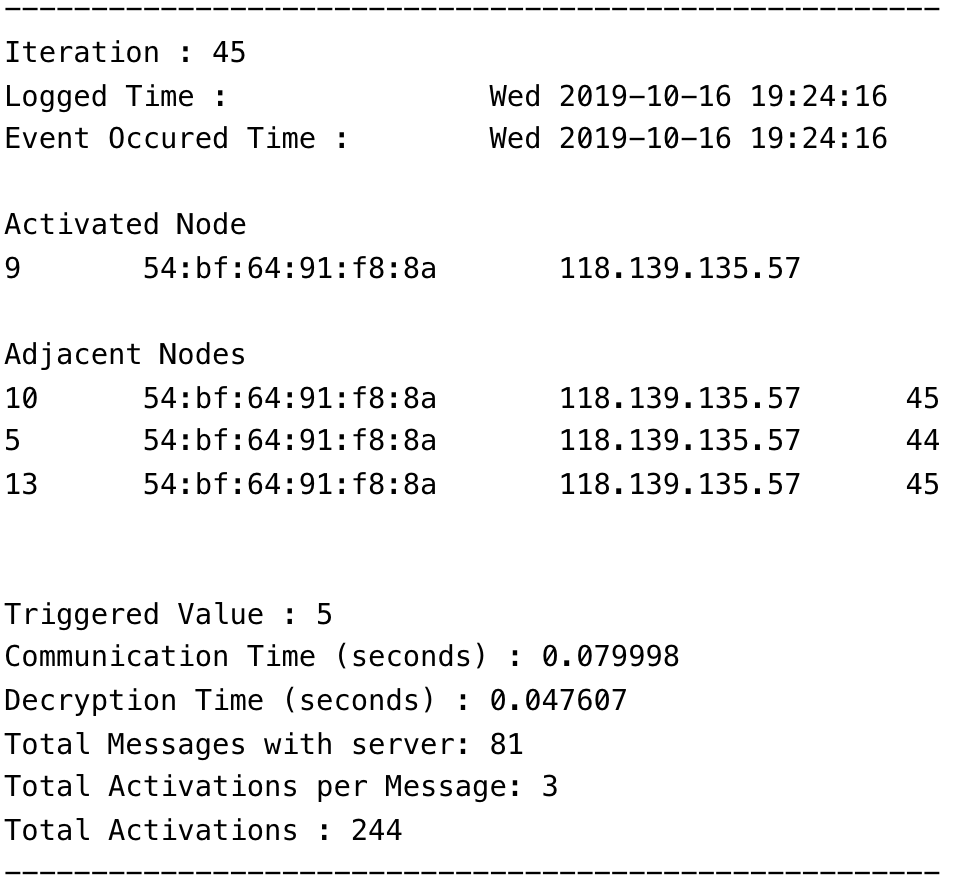
\includegraphics[width=3.3in,keepaspectratio]{logE}
		\caption{Base station log file for event details}
		\label{lst:log1}
	\end{figure}	
	Listing \ref{lst:log1} shows an event triggered at the 98 iteration of our test. This can be observed from the first line of the log which determines the iteration number. The next two lines of the logs displays the time when the event was logged on the file and the actual time when the event is detected respectively. This is useful when the node and base station is present in two geographical locations and the time to send the message effects the logging time. But in this example, since the node is a process inside the same machine, we are not able to see a difference. The next two lines denote the activated node that was triggered i.e. the node that sent the message to the base station. The Rank, MAC Address and IP Address of the activated node is being logged in the log file. In a case where each node were running on separate machines, we are able to see different MAC and IP addresses. Next the adjacent nodes which generated the same random number is being logged. Similar to the adjacent node the Rank, MAC Address and IP Address of the activated node is also being logged in the log file. But there is also a fourth item that stores the iteration number. Since the WSN takes into account the random values generated from the previous iteration, this value help to identify which in which iteration the same random number was generated.
	
	The next part of the log file shows the random number that triggered the event. Then the communication time and the decryption time is logged. The total messages with the base station shows how many messages are being sent to the server up until the current iteration. The total activations per message shows how many nodes are triggered for the current message. This can be either 3 or 4. Then finally the total activations up until the current iteration is also logged.
	

	
	Listing \ref{lst:log2} displays the log file that is generated at the end, when the system turns off gracefully. It records the total simulation time, total messages to the base station, total sensor node to sensor node messages and the total messages through the network. The total messages through the network contains the messages sent between the sensor nodes, messages sent from node to base station when an event is triggered and finally the messages sent from the  sensor nodes with the termination signal to stop gracefully.  It then also logs the total activations though out the network and how many times each node was activated during the simulation. 
	
	\begin{figure}[!h]
		\centering
		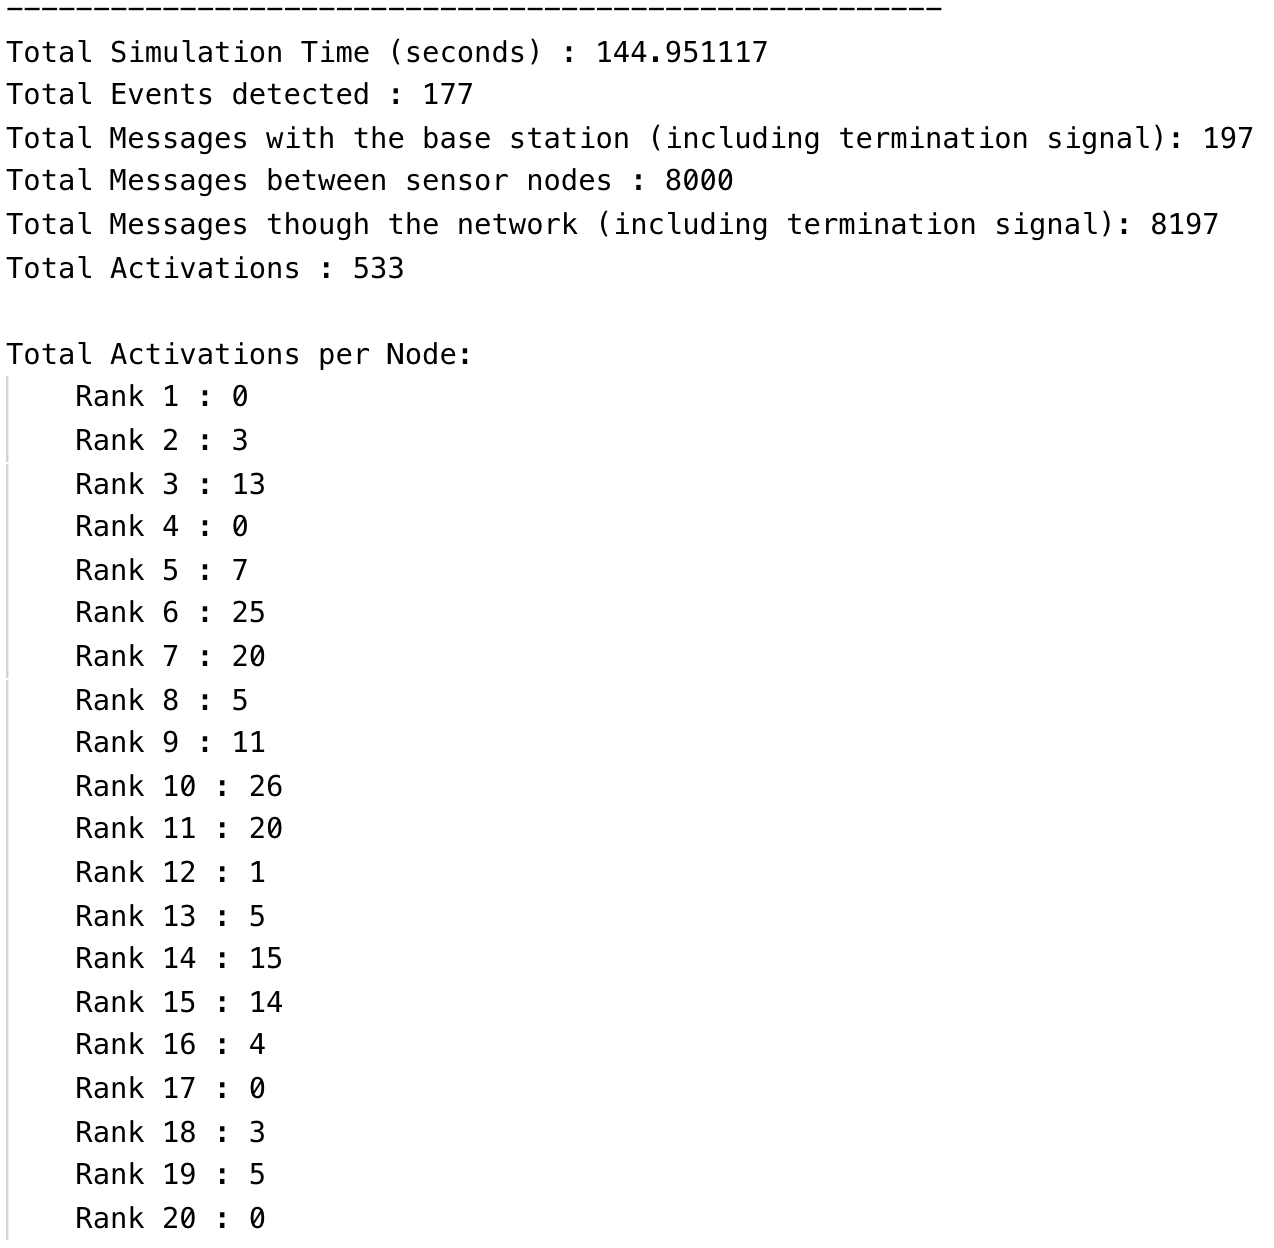
\includegraphics[width=3.3in,keepaspectratio]{logS}
		\caption{Base station log file for simulation details}
		\label{lst:log2}
	\end{figure}	
	
	\subsubsection{Sensor Node Log File}
	
	Next we look into the log file of each sensor node. Figure \ref{Message} shows the first event of the log file generated by the node with rank 6. This log file contains the original un-encrypted message, the encryption time and the encrypted message. If we analyze the log file we can see the time stamp in the original message but, after encrypting we do not see it. Do note the encryption time shown in Figure  \ref{Message} is not the encryption time used for the speed up analysis.
	
	\begin{figure}[!h]
		\centering
		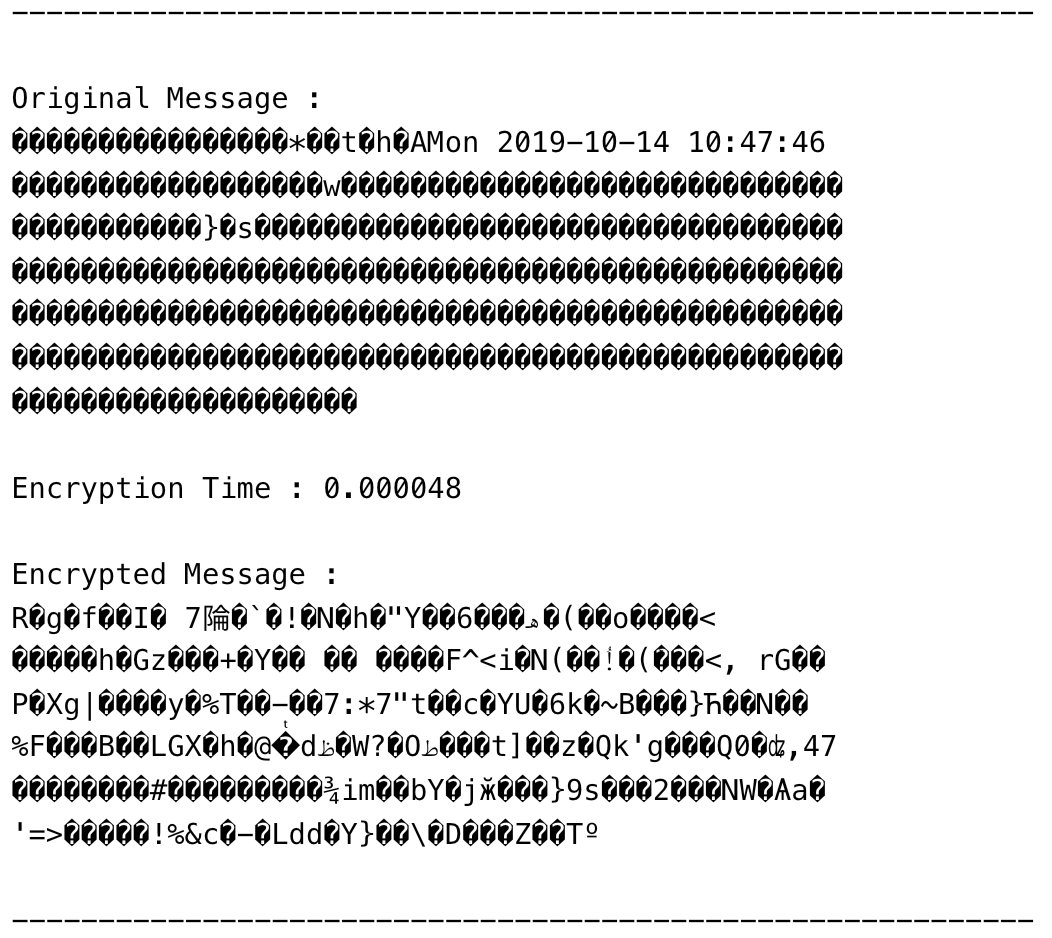
\includegraphics[width=3.3in,keepaspectratio]{en}
		\caption{Sensor Node log file}
		\label{Message}
	\end{figure}
	

	\subsection{Inter Process Communication Analysis}
	
	In this section we analyze the WSN data collected from the test case. We will explore the following sections of the data in this section.

	\subsubsection{Event detection messages from sensor nodes to base station}
	
		\begin{figure*}[!h]
		\centering
		\caption{Analysis of the data generated from the WSN}
		\subfloat[Total Messages per Iteration]
		{
			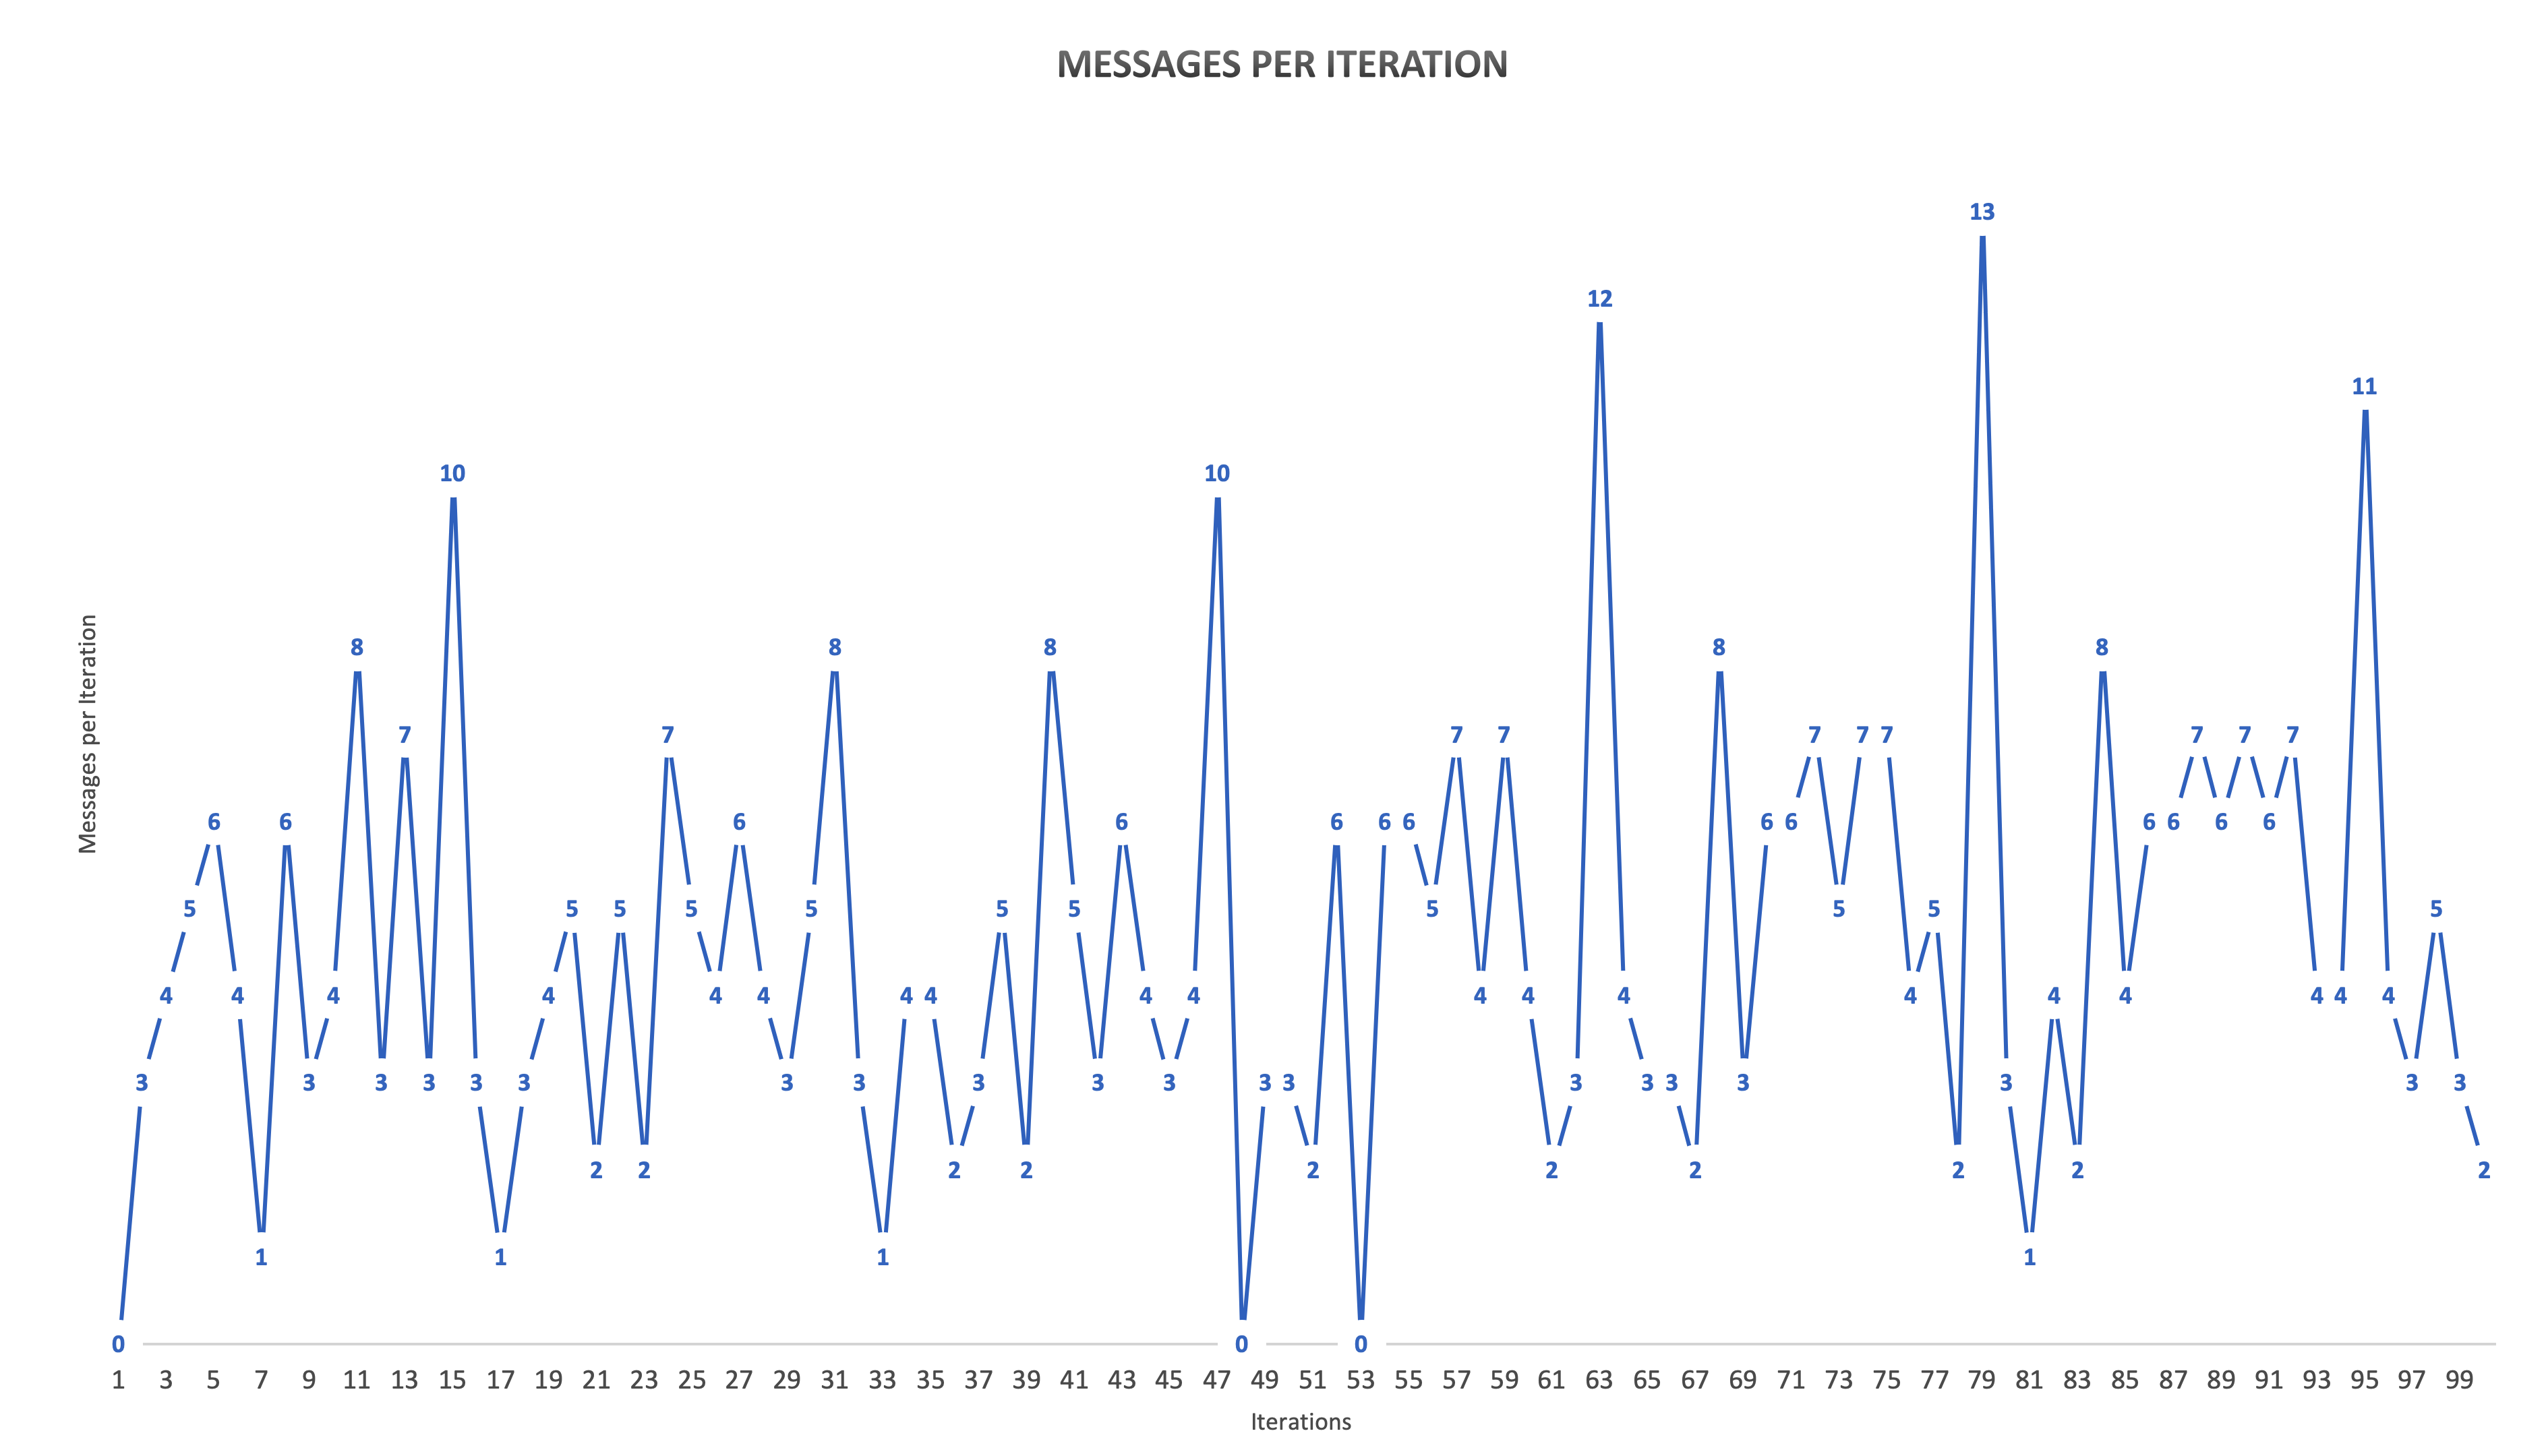
\includegraphics[width=4.5in]{chart1}
			\label{me}
		}
		\\
		\subfloat[Average Communication Time per Iteration]
		{
			
			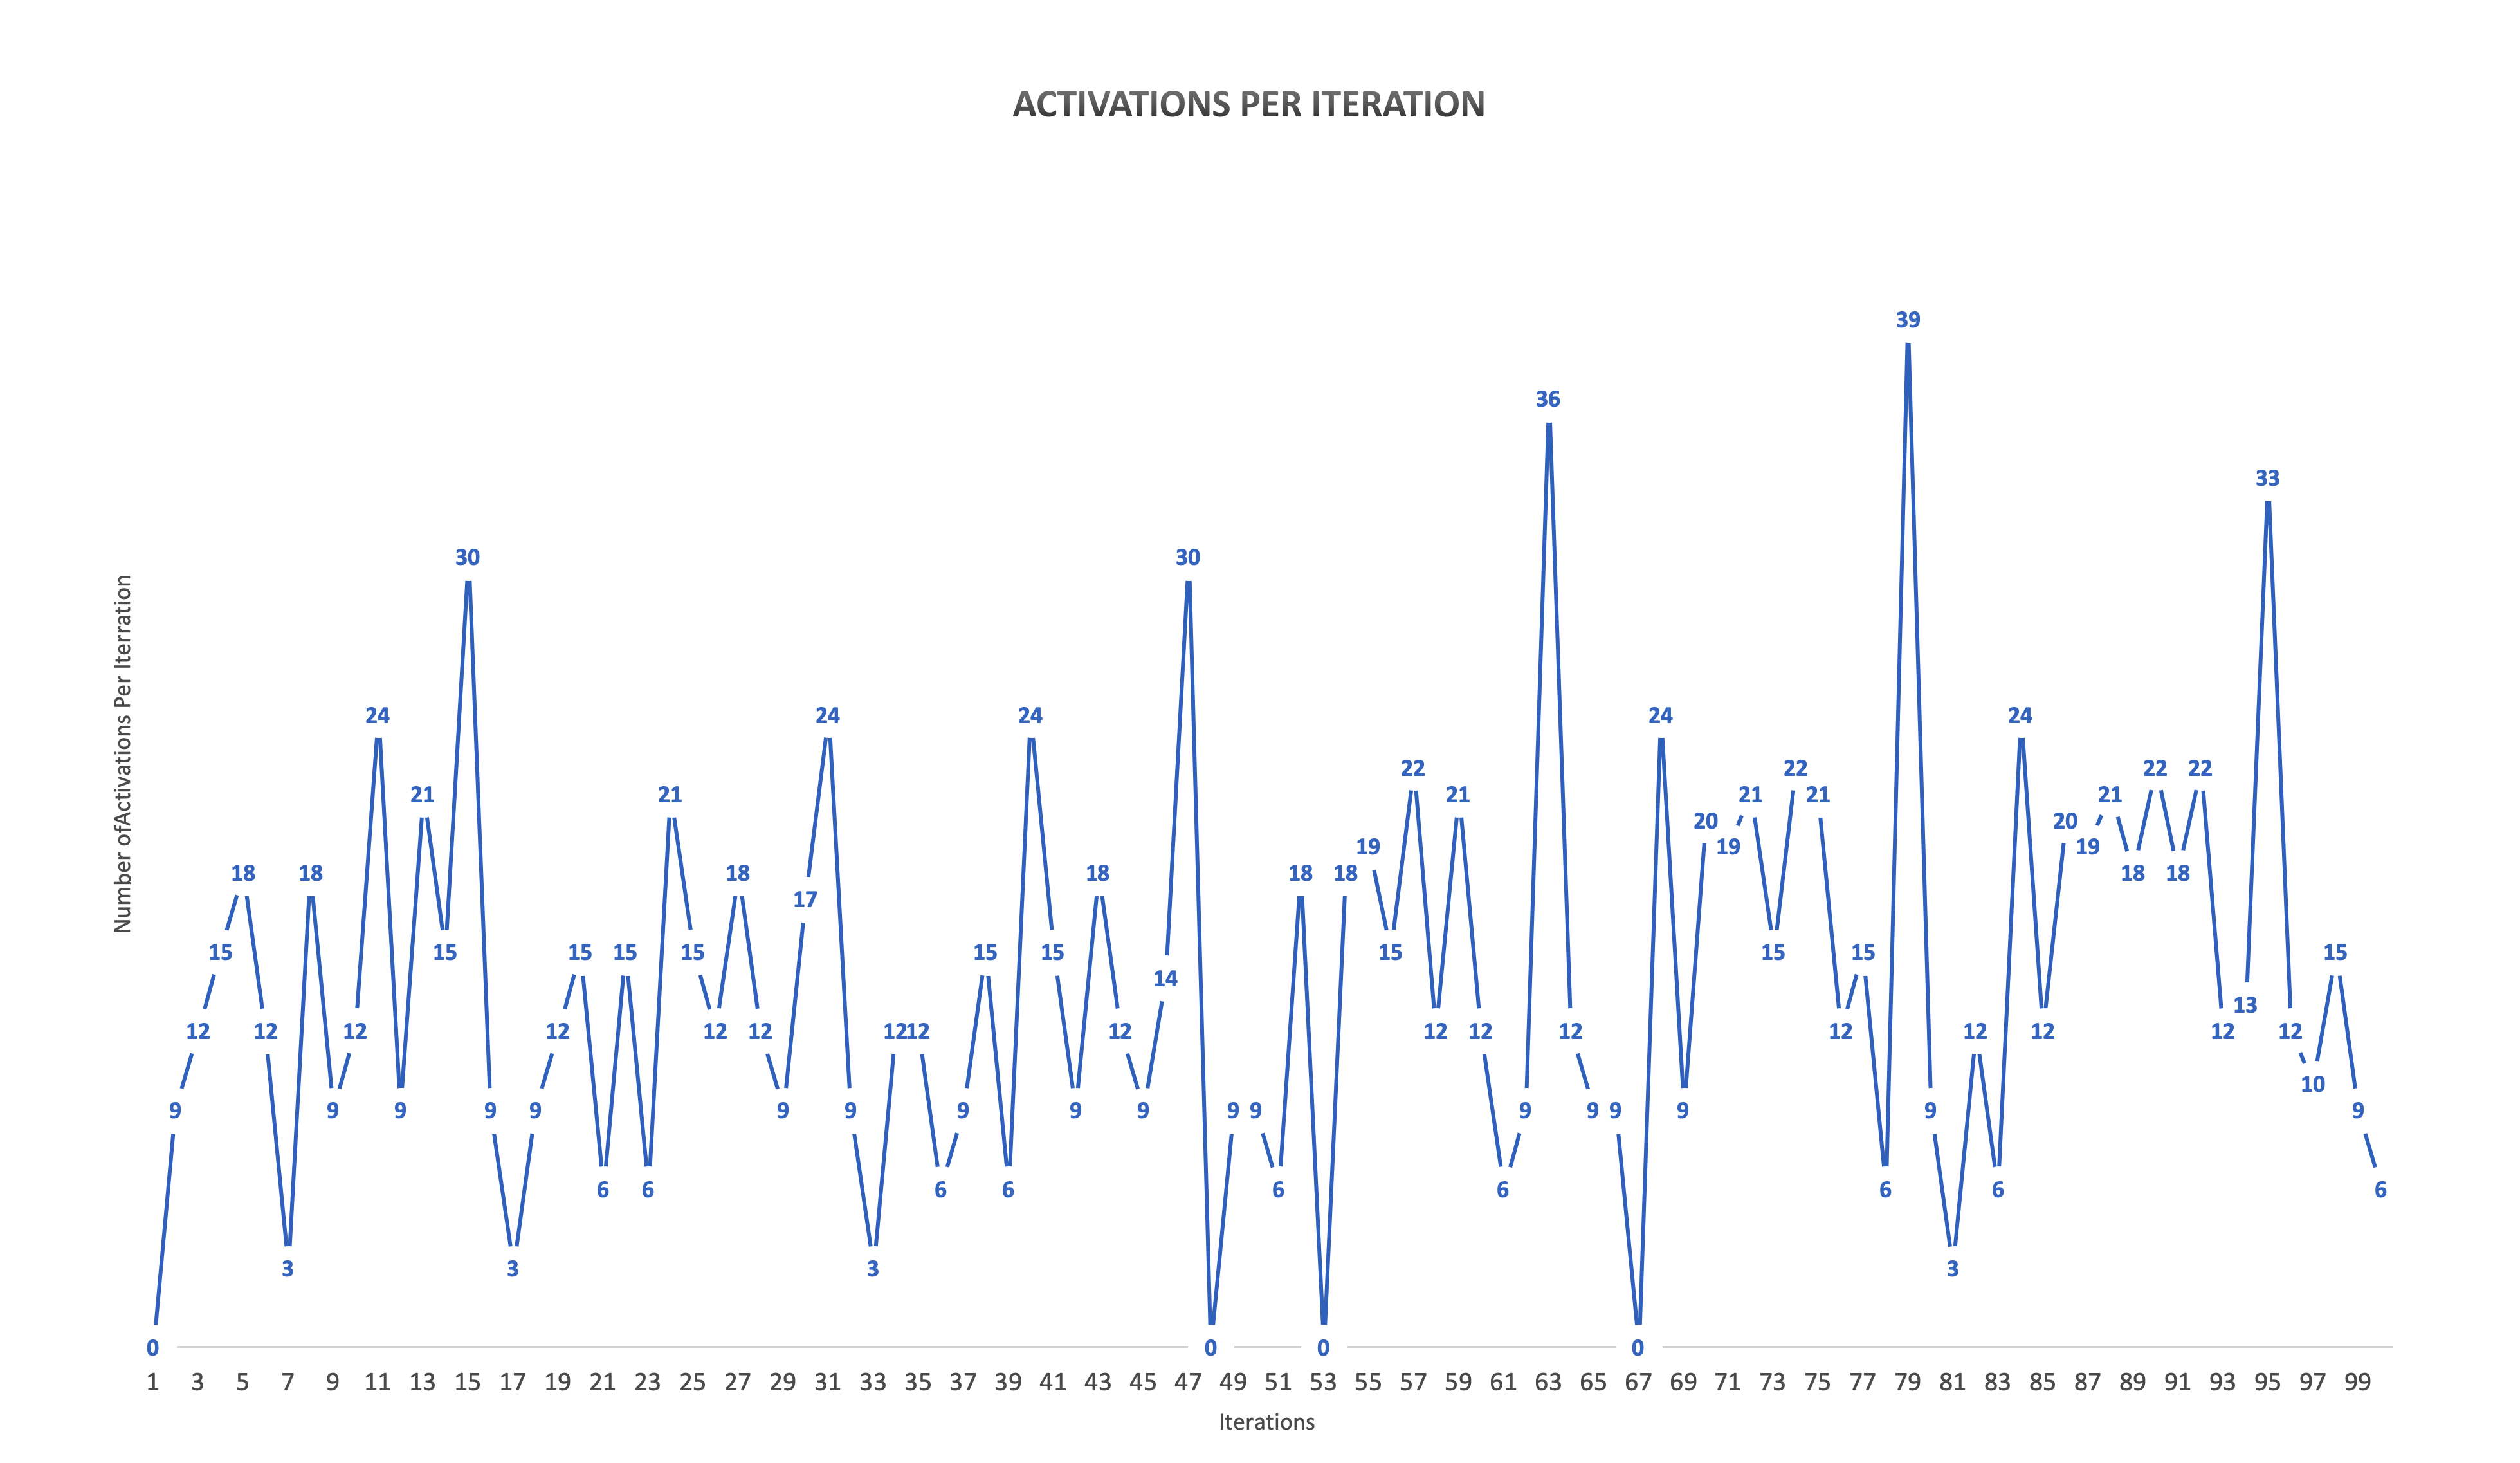
\includegraphics[width=4.5in]{chart2}
			\label{com}
		}
	\end{figure*}	

	 For each event detection, this architecture sends one message from the activated node to the base station. So referring to listing \ref{lst:log2}, the total number of events generated is 459 and the total number of messages received from the nodes to the server is 479 which includes the 20 termination signals sent at the end. Figure \ref{me} plots the number of messages received from the nodes over iterations. To highest number of messages of 13 out of the 20 nodes were received at iteration 79. We can also see that after every iteration that has a high number of messages, the number of messages plummets down. The reason for this is, commonly high number messages occur when there are matching random numbers in both the current iteration and the previous iteration. So after a high message iteration the previous array mostly contains 2 or more of the same common random numbers. So the probability of the random number of the current iteration being the same is low. Therefore the number of events detected in the next iteration goes down. Now referring  Figure \ref{act}, we see that it also follows the same pattern as Figure \ref{me}. But the counts is different as each message can have 3 or 4 activations.
	 
	 \begin{figure}[!h]
	 	\centering
	 	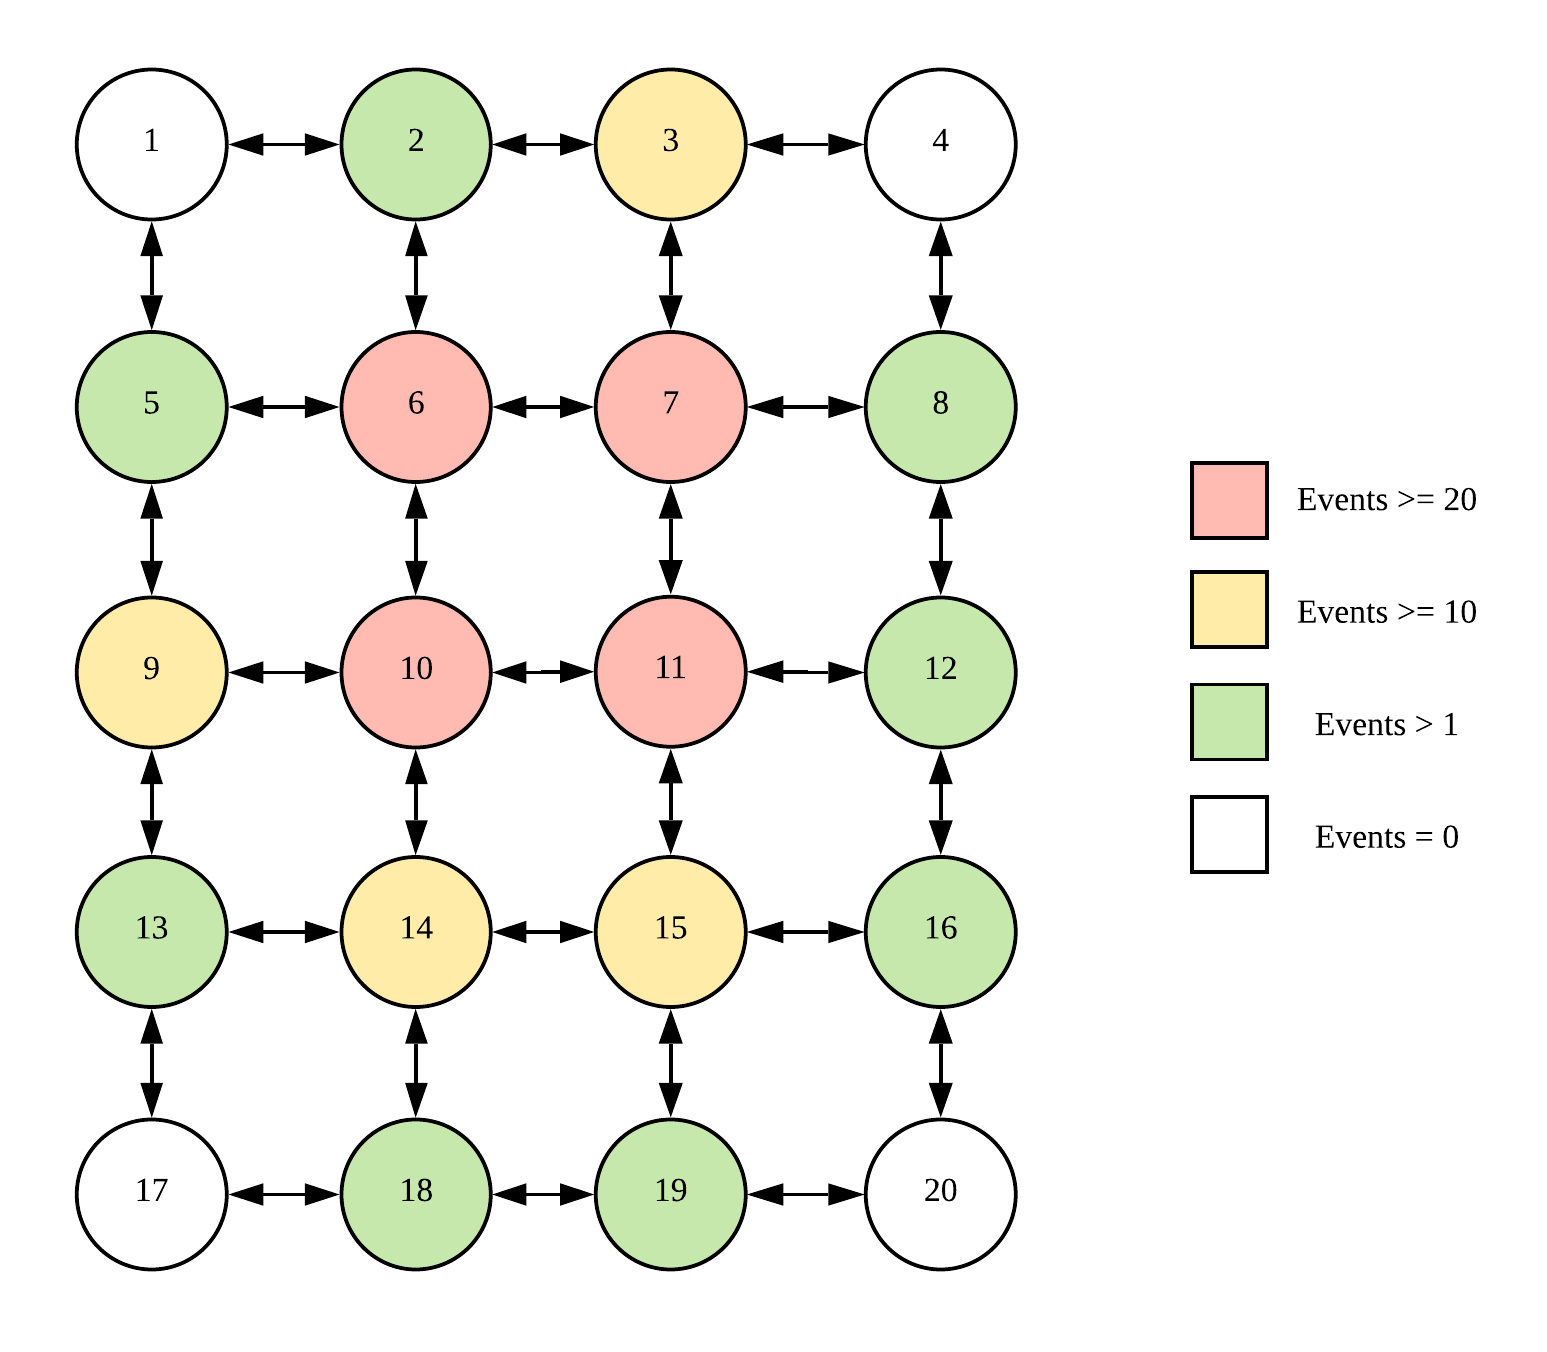
\includegraphics[width=3.in,keepaspectratio]{gridsum}
	 	\caption{Sensor Grid overlayed with the total event detection from each node}
	 	\label{colgrid}
	 \end{figure}
 
	\subsubsection{Total Events detected from each node}
	Next lets look at Figure \ref{colgrid}, which is a heat map of the nodes and the events detected from each of them. The sensor nodes with four adjacent neighbors have the highest number of events generated as it has more probability of having 3 or more common random number. Also note the four corner node never 
	detect an event as they only have 2 adjacent nodes. Therefore the observations satisfy the actual probability of the event detection.
	
	\subsubsection{Communication time}
	
	The communication time includes the time for encrypting the message, sending the message, receiving the message and decrypting the message. Since the tests case is run on a single computer, the communication time from node to node is similar except between iteration 55-70. This can be observed by Figure \ref{com}, where the is a peak in the average communication time. But if one part of the network is in a separate geographical location to the base station, the communication time will increase. The issue that arises with this is that the nodes with high communication time will take longer to finish the iterations. So the base station will wait until all the nodes have sent the termination signal to avoid any issue. One way to improve the communication time is by parallelizing the encryption and decryption algorithms which we will look into in the next section.

	\subsection{Encryption Analysis}	\label{encry}
	
		
	 \begin{figure}[!h]
	\centering
	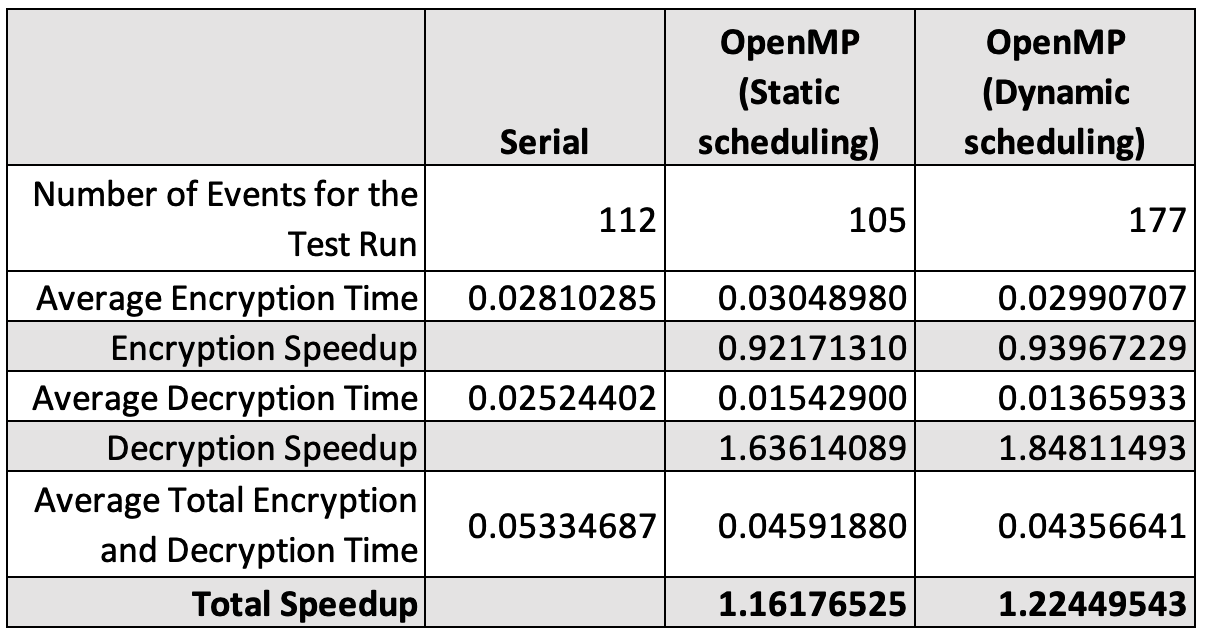
\includegraphics[width=3in,keepaspectratio]{speed}
	\caption{Analysis of the OpenMP speed up for encryption and decryption}
	\label{speedup}
	\end{figure}
	
	In this section we will analyze how OpenMP helps improve encryption and decryption time of the AES algorithm. Since we are using the CTR mode operation of the AES algorithm, the algorithm is parallelizable. 	The buffer size of the messages used for testing the encryption is different from the actual buffer size which was used to get the results. The reason for this is the smaller buffer size is insignificant to see any speed up when parallelizing the code as they are in microseconds. So for testing the speed up of the encryption and decryption we used a buffer size of 160000 initialized with zeros.
	
	In order to compare the speed up, first the encryption and decryption time of the AES algorithm without OpenMP is recorded. The encryption time is extracted from the node log files where as the decryption time extracted from the base station log file. 
	
	OpenMP has a static and dynamic way to parallelizing a for loop \ref{}. In order to determine which way better, average of two runs from each method are obtained and the speed is is calculated. This is done for both the encryption and decryption process with a pack size of 160000. Figure \ref{enTIme} and \ref{deTime}, shows the results obtained by the experiment and the static approach has a higher speed up for both encryption and decryption. The reason for this is that dynamic is better when the time taken for each iteration is not constant, but static is better when each iteration takes the same amount of time. Since each iteration of our loop is takes a constant time, the static approach is able to outperform the dynamic one. Therefore the WSN implementation uses the static approach.

	
	\section{Conclusion}
	
	\section{Future Work}
	
	Different grid architectures in different locations
	
	Prove the drop of events
	
	optimize the packsize to be dynamic based on the data sent
	
	

	
\bibliographystyle{IEEEtran}
\bibliography{ref.bib}

	\newpage
	\onecolumn
	\appendix
	
	
\begin{figure*}[h]
	\centering
	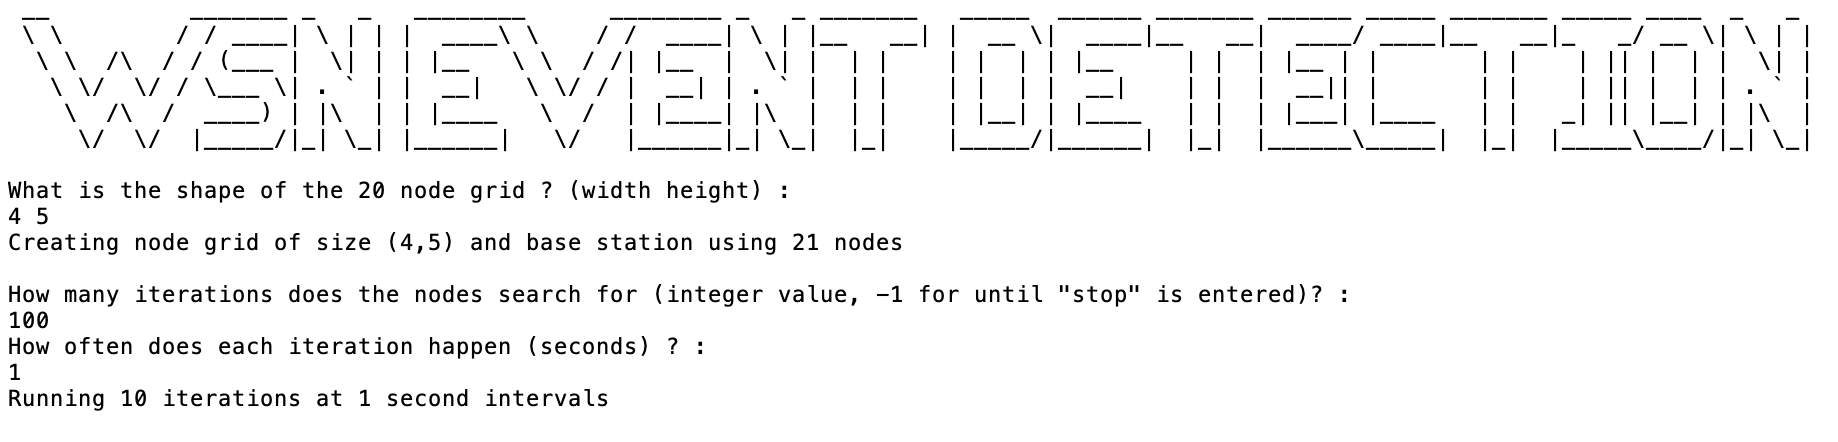
\includegraphics[width=6in,keepaspectratio]{console1}
	\caption{Screenshot of the console used for the generating the results}
	\label{screen 1}
\end{figure*}

\begin{figure*}[h]
	\centering
	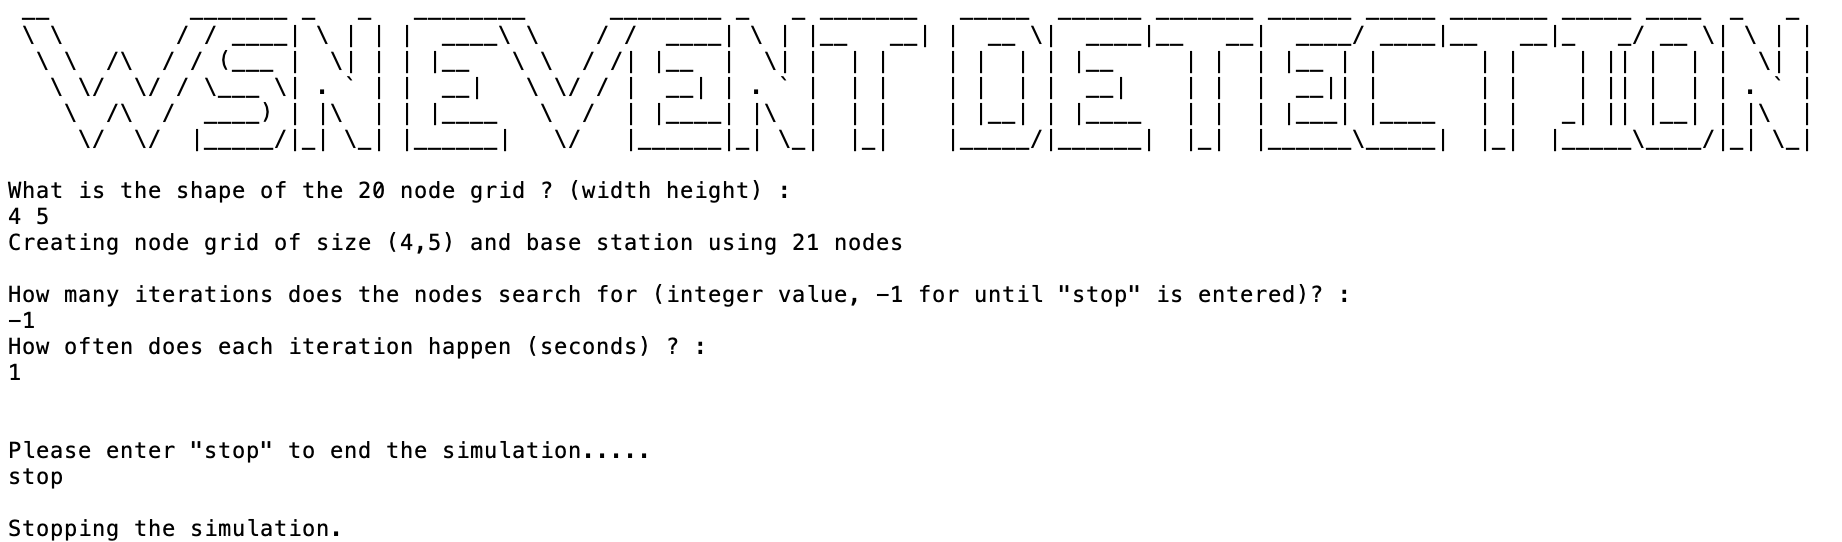
\includegraphics[width=6in,keepaspectratio]{console2}
	\caption{Screenshot of the alternative approach to run the program until user enters stop}
	\label{screen 2}
\end{figure*}

\end{document}
